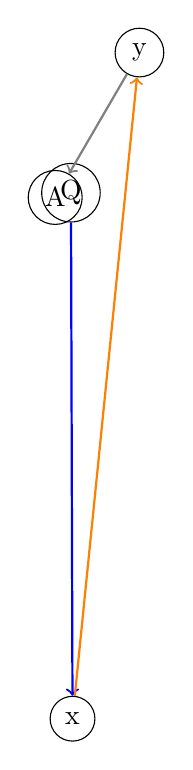
\begin{tikzpicture}
\node[circle, draw=black] (a) at (-3.01, 2.40) {Q};
\node[circle, draw=black] (b) at (-2.99, -4.28) {x};
\node[circle, draw=black] (c) at (-2.14, 4.18) {y};
\node[circle, draw=black] (d) at (-3.21, 2.34) {A};
\draw[->, thick, blue] (a) -- (b);
\draw[->, thick, orange] (b) -- (c);
\draw[->, thick, gray] (c) -- (d);
\end{tikzpicture}